\documentclass[11pt,a4paper]{article}
\usepackage[utf8]{inputenc}
\usepackage{float,graphicx,amsfonts,amsmath,amssymb,authblk,graphicx,longtable,booktabs,fullpage}
\usepackage{wrapfig}
\graphicspath{ {../img/} }
\usepackage[colorlinks = true,
            linkcolor = black,
            urlcolor  = blue,
            citecolor = blue,
            anchorcolor = blue]{hyperref}


\title{
  Misura della distanza focale di una lente convergente \vspace{1em} \\
  \large  Esame di Laboratorio di Fisica 2 \\
  \small prof. Salvatore Costa
  }
    

\author[1]{Dennis Angemi}%
\affil[1]{Dipartimento di Fisica e Astronomia ``Ettore Majorana'', Università degli Studi di Catania}%
\date{17 giugno 2023}

\begin{document}

\maketitle

\section{Introduzione}
\subsection{Scopo della misura}
L'esperienza ha l'obiettivo di misurare la distanza focale $f$ di una lente convergente ed esprimere la potenza di tale lente in diottrie, adoperando un banco ottico. Inoltre sono stati misurati gli ingrandimenti prodotti dalla lente in diverse configurazioni.

\subsection{Cenni teorici}

Una lente è un corpo trasparente, con un indice di rifrazione $n$, limitato da due superfici curve o da una superficie piana e una superficie curva, che è in grado di modificare la traiettoria di un raggio luminoso che lo attraversa. Quando un raggio luminoso si avvicina a una lente, subisce due rifrazioni: la prima avviene quando passa dal mezzo in cui si propaga, generalmente aria, al mezzo in cui è costituita la lente; la seconda avviene quando il raggio luminoso passa da quest'ultimo mezzo al mezzo successivo, di solito ancora aria.
\\
Nel seguito di questo studio, verranno considerate lenti di spessore trascurabile e si sfrutterà perciò l'approssimazione della lente sottile per cui si assume che il raggio luminoso venga deviato una sola volta durante il passaggio attraverso la lente.
\\
L'esperienza in questione ha fatto uso di una lente convergente: una tipologia di lenti che sono riconoscibili per la loro forma più spessa al centro e più sottile ai bordi; le lenti divergenti sono più spesse ai bordi e più sottili al centro.
\\
Se la lente, come abbiamo assunto, è sottile, per essa vale la relazione
\begin{equation}
    \frac{1}{p}+\frac{1}{q} = (n - 1) \left(\frac{1}{R_1} - \frac{1}{R_2}\right)
\end{equation}
in cui:
\begin{itemize}
    \item $p$ e $q$ rappresentano rispettivamente le distanze oggetto-lente e lente-immagine;
    \item $R_1$ e $R_2$ indicano i raggi di curvatura delle superfici sferiche che compongono la lente.
    \item $n$ rappresenta l'indice di rifrazione del materiale che costituisce la lente.
\end{itemize}
Il prodotto 
$$(n - 1)\left(\frac{1}{R_1} - \frac{1}{R_2}\right)$$
è una costante il cui reciproco viene indicato con $f$ e che prende il nome di distanza focale. È  possibile dunque riscrivere la relazione precedente in questa forma che va sotto il nome di legge dei punti coniugati.
\begin{equation}
    \frac{1}{p}+\frac{1}{q}=\frac{1}{f}
    \label{eq:punti-coniugati}
\end{equation}

\section{Descrizione dell’ apparato sperimentale}
Nell'esecuzione delle misure è stato utilizzato un banco ottico, schematizzato in Figura \ref{fig:exp}, che è composto da un binario dotato di regolo che consente di leggere le posizioni degli oggetti su di esso collocati. Nel dettaglio, sono stati utilizzati:

\begin{itemize}
    \item Un proiettore che funge da sorgente luminosa;
    \item Una lamina sottile con una fenditura che funge da oggetto;
    \item Una lente convergente biconvessa
    \item Uno schermo che viene utilizzato per visualizzare l'immagine prodotta dalla rifrazione dei raggi che attraversano la lente
\end{itemize}

La fenditura, la lente e lo schermo sono posizionati su  appositi supporti che consentono loro di scorrere sul banco e di essere fissati tramite viti.

\begin{figure}[H]
    \centering
    \includegraphics[width=0.7\textwidth]{img/esperimento.png}
    \caption{Banco ottico}
    \label{fig:exp}
\end{figure}

\subsection{Principio di funzionamento degli apparecchi}

Per l'acquisizione delle misure delle posizioni è stato utilizzato regolo di sensibilità 1 mm è uno strumento di misura utilizzato per determinare la lunghezza di oggetti con una precisione di 1 millimetro. Per effettuare la lettura di una misura, è stato sufficiente individuare la posizione della tacca situata in corrispondenza dei supporti sul banco ottico.
\\ \\
L'acquisizione delle lunghezze dell'oggetto invece è stata possibile grazie a un calibro ventesimale che è uno strumento composto da una coppia di ganasce mobili che si possono allargare o stringere per adattarsi alle dimensioni dell'oggetto da misurare. La scala graduata del calibro mostra le misure in centimetri e i suoi meccanismi consentono una regolazione molto precisa della distanza tra le ganasce per ottenere una misura accurata.
\\
Il proiettore emette un fascio di luce che viene diretto su di una lastra metallica.

\subsection{Caratteristiche degli strumenti di misura}
Di seguito si allega la sensibilità dei due unici strumenti di misura che sono stati adoperati durante l'esecuzione dell'esperienza
\begin{longtable}[]{@{}ll@{}}
    \toprule
    Strumento & Sensibilità \tabularnewline
    \midrule
    \endhead
    Calibro ventesimale & 0.005 $\; cm$ \tabularnewline
    Regolo & 0.1 $\; cm$ \tabularnewline
    \bottomrule
    \label{tab:tools}
    \\
    \caption{Strumenti adoperati}
\end{longtable}

\section{Esecuzione dell’esperienza}

\subsection{Procedura}
L'esperienza consiste nell'acquisizione di 3 serie di misure la cui procedura è di seguito riassunta.

\subsubsection{Prima configurazione}

Avendo acceso il proiettore P, che costituisce la sorgente luminosa utilizzata nell'esperimento, si è fissato l'oggetto O (che consiste in una incisione di una lastra metallica) in prossimità della sorgente (vd. Tabella \ref{tab:conf1}). Successivamente sono state ripetute le seguenti azioni per 10 iterazioni: dopo aver fissato la lente L ad una distanza arbitraria $p$ dall'oggetto (vd. Tabella \ref{tab:dconf1}) è stata modificata la posizione dello schermo S finché, su di esso, non si è osservata nitida l'immagine dell'oggetto illuminato. Per tale configurazione, sono state misurate le posizioni $p$ e $q$ leggendo le posizioni di oggetto, lente e schermo tramite il regolo del banco ottico (vd. Tabella \ref{tab:tools}). È stato inoltre utilizzato un calibro (vd. Tabella \ref{tab:tools}) per misurare la lunghezza dell'oggetto illuminato $i$ e dell'immagine $o$.

\subsubsection{Metodi di Bessel}
La seconda serie di misure sono state acquisite in una configurazione differente, infatti lente e schermo sono stati posizionati inizialmente vicino all'oggetto. Successivamente, mantenendo invariata la posizione della piastra metallica che costituisce l'oggetto, lo schermo e la lente sono stati allontanati gradualmente, in modo da verificare la condizione per cui la distanza oggetto-lente coincidesse con la distanza lente-schermo la condizione per cui la lunghezza dell'immagine coincidesse con quella dell'oggetto. Per tale configurazione è stata acquisita la misura della distanza minima $D$ tra oggetto e schermo per cui l'immagine sullo schermo è apparsa nitida

\subsubsection{Errori sistematici}
Infine, per indagare la presenza di eventuali errori sistematici sono stati fissati 11 valori della distanza oggetto-schermo e sono state misurate le distanze $s$ e $d$ che indicano rispettivamente le distanze tra il punto medio di $D$ e gli estremi dell'intervallo delle posizioni della lente per cui si produce un'immagine ugualmente nitida sullo schermo (vd. Tabella \ref{tab:dconf3}

\subsection{Dati sperimentali}

\subsubsection{Dettagli fenditura}
La lunghezza $o$ dell'incisione sulla lastra metallica, misurata con un calibro ventesimale è
\begin{equation}
    o = 1.850 \pm 0.005 \; cm
\end{equation}

\subsubsection{Prima configurazione}
Durante l'acquisizione della prima serie di misure, i valori della Tabella \ref{tab:conf1} sono rimasti invariati.
\begin{longtable}[]{@{}lll@{}}
    \toprule
    configuration & $x_p \; [cm]$ & $x_o \; [cm]$ \tabularnewline
    \midrule
    \endhead
    1 & 4.60 $\pm \; 0.05$ & 10.10 $\pm \; 0.05$ \tabularnewline
    \bottomrule
    \label{tab:conf1}
    \\
    \caption{Configurazione 1}
\end{longtable}
    
dove
\begin{itemize}
    \item $x_p$ rappresenta la posizione del proiettore;
    \item $x_o$ rappresenta la posizione dell'oggetto;
\end{itemize}

\begin{longtable}[]{@{}llllll@{}}
    \toprule
    Measure ID & $x_l$ & $x_{s,inf}$ & $x_{s,sup}$ & $l_{inf}$ & $l_{sup}$ \tabularnewline
     & $\pm \; 0.05 \; cm$ & $\pm \; 0.05 \; cm$ & $\pm \; 0.05 \; cm$ & $\pm \; 0.005 \; cm$ & $\pm \; 0.005 \; cm$ \tabularnewline
    \midrule
    \endhead
    C1M1 & 21.80 & 66.30 & 78.40 & 6.360 & 7.850 \tabularnewline
    C1M2 & 22.50 & 60.40 & 65.90 & 5.090 & 6.230 \tabularnewline
    C1M3 & 23.00 & 59.90 & 64.90 & 5.065 & 6.095 \tabularnewline
    C1M4 & 23.50 & 56.85 & 58.90 & 4.235 & 4.850 \tabularnewline
    C1M5 & 24.00 & 55.30 & 56.80 & 3.985 & 4.320 \tabularnewline
    C1M6 & 24.50 & 53.70 & 54.30 & 3.600 & 3.275 \tabularnewline
    C1M7 & 24.80 & 52.85 & 54.50 & 3.265 & 3.890 \tabularnewline
    C1M8 & 25.00 & 52.80 & 53.80 & 3.410 & 3.535 \tabularnewline
    C1M9 & 25.30 & 51.90 & 53.00 & 3.150 & 3.995 \tabularnewline
    C1M10 & 25.50 & 51.60 & 52.80 & 3.000 & 3.285 \tabularnewline
    \bottomrule
    \label{tab:dconf1}
    \\
    \caption{Dati grezzi configurazione 1}
\end{longtable}

dove
\begin{itemize}
    \item $x_l$ rappresenta la posizione della lente;
    \item $x_{s,inf}$ e $x_{s,inf}$ rappresentano rispettivamente la posizione dell'estremo inferiore de di quello superiore dell'intervallo in cui l'immagine appare nitida sullo schermo;
    \item $l_{inf}$ e $l_{sup}$ rappresentano rispettivamente l'estremo inferiore e superiore dell'intervallo delle lunghezze dell'immagine della fenditura per cui essa fosse nitida;
\end{itemize}

\subsubsection{Seconda configurazione}
Metodo di Bessel

\begin{longtable}[]{@{}llllll@{}}
    \toprule
    Measure ID & $x_p$ & $x_o$ & $x_l$ & $x_s$ &  $l$ \tabularnewline
      & $\pm \; 0.1 \; cm$ & $\pm \; 0.1 \; cm$ & $\pm \; 0.1 \; cm$ & $\pm \; 0.1 \; cm$ & $\pm \; 0.005 \; cm$ \tabularnewline
    \midrule
    \endhead
    C2M1 & 4.6 & 10.0 & 29.8 & 49.6 & 1.850 \tabularnewline
    \bottomrule
    \label{tab:dati-bessel}
    \\
    \caption{Dati grezzi configurazione 2}
\end{longtable}

dove
\begin{itemize}
    \item $x_p$, $x_o$, $x_l$, $x_s$ rappresentano rispettivamente la posizione del proiettore, dell'oggetto, della lente e dello schermo
    \item $l$ rappresenta la lunghezza dell'immagine
\end{itemize}

\subsubsection{Terza configurazione}
Indagine su eventuali errori sistematici
\\
Durante l'acquisizione della terza serie di misure si è mantenuta costante la posizione dell'oggetto $x_o = 10.10 \pm 0.05 \; cm$.

\begin{longtable}[]{@{}llll@{}}
    \toprule
    Measure ID & $x_s$ & $x_{l1}$ & $x_{l2}$ \tabularnewline
      & $\pm \; 0.05 \; cm$ & $\pm \; 0.05 \; cm$ & $\pm \; 0.05 \; cm$ \tabularnewline
    \midrule
    \endhead
    C3M1 & 54.00 & 24.15 & 38.90 \tabularnewline
    C3M2 & 54.50 & 24.35 & 39.05\tabularnewline
    C3M3 & 55.00 & 24.65 & 39.65\tabularnewline
    C3M4 & 55.50 & 24.25 & 40.20\tabularnewline
    C3M5 & 56.00 & 23.90 & 40.85\tabularnewline
    C3M6 & 56.50 & 24.05 & 40.65\tabularnewline
    C3M7 & 56.70 & 24.10 & 41.70\tabularnewline
    C3M8 & 57.00 & 24.15 & 42.10\tabularnewline
    C3M9 & 57.30 & 24.00 & 42.25\tabularnewline
    C3M10 & 57.50 & 24.10 & 42.85\tabularnewline
    C3M11 & 57.80 & 23.95 & 43.05\tabularnewline
    \bottomrule
    \label{tab:dconf3}
    \\
    \caption{Dati grezzi configurazione 3}
\end{longtable}

dove
\begin{itemize}
    \item $x_s$ rappresenta la posizione dello schermo S
    \item $x_{l1}$ e $x_{l2}$ rappresentano rispettivamente gli estremi inferiori e superiori degli intervalli della posizione della lente convergente per cui si osservava nitidamente l'immagine sullo schermo S.
\end{itemize}




\section{Analisi dei dati}
\subsection{A}
\subsubsection{Stima di $f$ da media pesata}
Avendo a disposizione le misure delle posizioni di oggetto, lente e schermo (Tabelle \ref{tab:conf1} e \ref{tab:dconf1}) procedo alla determinazione delle grandezze $p$ e $q$ già introdotte nell'eq. \ref{eq:punti-coniugati} calcolando le seguenti distanze
\\
\begin{equation}
    \qquad{p = |x_o - x_l|}
    \qquad{q = |x_i - x_l|}
    \label{eq:pq-calculated}
\end{equation}
dove
\begin{equation}
    x_i = \frac{x_{s,inf} + x_{s,sup}}{2}
\end{equation}
\\
rappresenta la media delle posizioni occupate dallo schermo nell'intervallo $[x_{s,inf},x_{s,sup}]$ in cui è possibile distinguere l'immagine nitidamente. A tale posizione $x_i$, si conferisce la seguente incertezza pari al semi-intervallo precedentemente introdotto
\begin{equation}
    \delta x_i = \frac{|x_{s,inf} - x_{s,sup}|}{2}.
\end{equation}
Infine, alle distanze oggetto-lente e lente-immagine si attribuiscono le incertezze
\begin{equation}
    \qquad{\delta p = 2\delta s}
    \qquad{\delta q = \sqrt{(\delta s)^2 + (\delta x_i)^2}}
    \label{eq:dpdq}
\end{equation}
Essendo $\delta s = \frac{1}{2} \; mm$ cioè pari alla sensibilità di lettura; si è ritenuto infatti ragionevole riuscire a discriminare una misura derivante dalla lettura dell'indice posizionato tra due tacche di ampiezza $1 \; mm$. I valori di $p$ e $q$ determinati tramite le eq. \ref{eq:pq-calculated} e \ref{eq:dpdq} sono riportati in tabella \ref{tab:pqf} insieme alle distanze focali stimate come nel seguito descritto. 
\\
È infatti possibile determinare la distanza focale $f$ in modo diretto usando la relazione
\\
\begin{equation}
    \frac{1}{p}+\frac{1}{q}=\frac{1}{f_d} \Rightarrow f_d=\frac{p q}{p+q}
    \label{eq:f-direct}
\end{equation}
\\
L'incertezza su tale grandezza sarà 
\\
\begin{equation}
    \delta f_d=\sqrt{\left(\frac{\partial f_d}{\partial p} \delta p\right)^2+\left(\frac{\partial f_d}{\partial q} \delta q\right)^2}
\end{equation}
\\
con
\\
\begin{equation}
    \qquad{\frac{\partial f_d}{\partial p}=\left(\frac{q}{p+q}\right)^2}
    \qquad{\frac{\partial f_d}{\partial q}=\left(\frac{p}{p+q}\right)^2}
\end{equation}
\\
per cui
\\
\begin{equation}
    \delta f_d=\sqrt{\left[\left(\frac{q}{p+q}\right)^2 \delta p\right]^2+\left[\left(\frac{p}{p+q}\right)^2 \delta q\right]^2}.
\end{equation}
\\
Di seguito si riportano i valori di $p$, $q$, $f_d$
\\
\begin{longtable}{@{}llll@{}}
\toprule
Measure ID & $p \pm \delta p$ & $q \pm \delta q$ & $f_d \pm \delta f_d$ \tabularnewline
\midrule
C1M1 & $11.7 \pm 0.1$ & $51 \pm 6$ & $9.5 \pm 0.2$ \tabularnewline
C1M2 & $12.4 \pm 0.1$ & $41 \pm 3$ & $9.5 \pm 0.2$ \tabularnewline
C1M3 & $12.9 \pm 0.1$ & $39 \pm 3$ & $9.7 \pm 0.2$ \tabularnewline
C1M4 & $13.4 \pm 0.1$ & $34 \pm 1$ & $9.6 \pm 0.1$ \tabularnewline
C1M5 & $13.9 \pm 0.1$ & $32.0 \pm 0.8$ & $9.70 \pm 0.08$ \tabularnewline
C1M6 & $14.4 \pm 0.1$ & $29.5 \pm 0.3$ & $9.68 \pm 0.06$ \tabularnewline
C1M7 & $14.7 \pm 0.1$ & $28.9 \pm 0.8$ & $9.7 \pm 0.1$ \tabularnewline
C1M8 & $14.9 \pm 0.1$ & $28.3 \pm 0.5$ & $9.76 \pm 0.07$ \tabularnewline
C1M9 & $15.2 \pm 0.1$ & $27.2 \pm 0.6$ & $9.74 \pm 0.08$ \tabularnewline
C1M10 & $15.4 \pm 0.1$ & $26.7 \pm 0.6$ & $9.77 \pm 0.09$ \tabularnewline
\bottomrule
\label{tab:pqf}
\\
\caption{Distanze focali determinate tramite la eq. \ref{eq:f-direct}}
\end{longtable}

Delle 10 misure di $f_d$ si è scelto di calcolare la media pesata $\bar{f_d}$ e la sua incertezza $\delta \bar{f_d}$
\\
\begin{equation}
    \qquad{\bar{f_d} = \frac{\sum_{i=1}^{10} w_i f_{d,i}}{\sum_{i=1}^{10} w_i }}
    \qquad{\delta \bar{f_d} = \sqrt{\frac{1}{\sum_{i=1}^{10} w_i}}}
    \label{eq:media-pesata-f}
\end{equation}
\\
essendo i pesi
\\
\begin{equation}
    w_i = \frac{1}{(\delta f_{d,i})^2}
\end{equation}
da cui si conclude
\begin{equation}
    \bar{f_d} = 9.70 \pm 0.03 \; cm
    \label{eq:f-diretta-media-pesata}
\end{equation}
\begin{figure}[H]
    \centering
    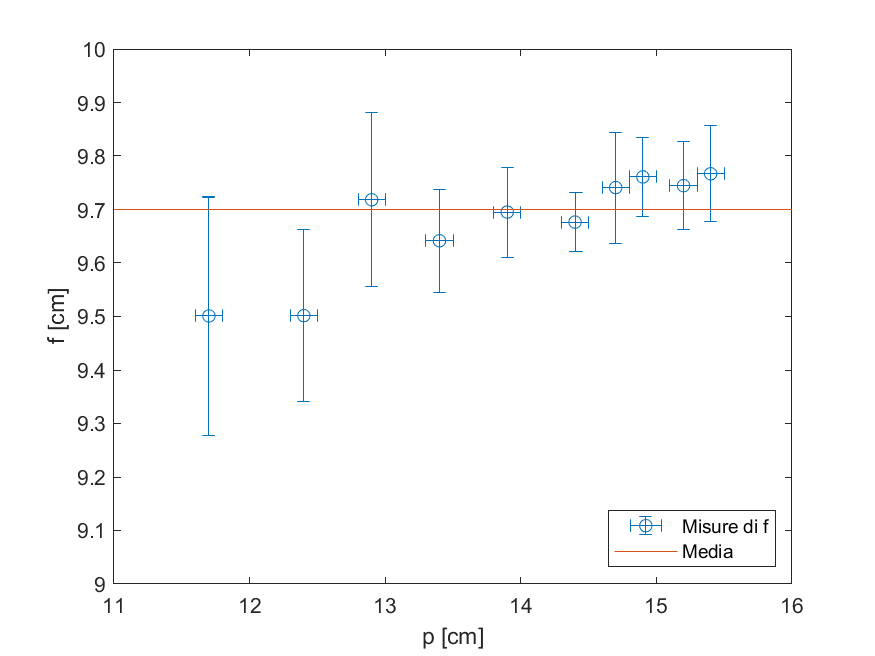
\includegraphics[scale = .7]{pf.png}
    \caption{Calcolo diretto della distanza focale $f$}
    \label{fig:pf}
\end{figure}

Come è possibile osservare dalla Figura \ref{fig:pf}, tutti gli intervalli di incertezza di $f_d \pm \delta f_d$ risultano compatibili con la media pesata $\bar{f_d} \pm \delta \bar{f_d}$ (rappresentata dalla banda arancione).

\subsubsection{Stima di $f$ tramite best-fit lineare}
Linearizziamo la legge dei punti coniugati l'equazione \ref{eq:punti-coniugati} 
\begin{equation}
    \frac{1}{p}+\frac{1}{q}=\frac{1}{f} \Longleftrightarrow \frac{1}{q} = \frac{1}{f} - \frac{1}{p}
    \label{eq:pqf-linearized}
\end{equation}
nella forma
\begin{equation}
    y = A + Bx
    \label{eq:retta-generica}
\end{equation}
avendo effettuato le seguenti posizioni:
\begin{equation}
    \qquad{x = \frac{1}{p}}
    \qquad{y = \frac{1}{q}}.
    \label{eq:xy}
\end{equation}
Applicando le relazioni \ref{eq:xy} ai valori di $p$ e $q$ della tabella \ref{tab:pqf}, si ottengono le coordinate $(x,y)$ dei punti di cui nel seguito indagheremo la correlazione lineare. A questi ultimi sono state conferite le incertezze propagando l'errore sul reciproco della distanza oggetto-lente e lente-immagine in tal modo:
\\
\begin{equation}
    \qquad{\delta x = \left | \frac{\partial x}{\partial p} \delta p \right | = \frac{\delta p}{p^2}} \; ,
    \qquad{\delta y = \left | \frac{\partial y}{\partial q} \delta q \right | = \frac{\delta q}{q^2}}
\end{equation}
\\
Essendo $\delta p$ e $\delta q$ stati determinati tramite la relazione \ref{eq:dpdq}. Si riportano appresso i valori determinati come sopra indicato.
\\
\begin{longtable}[]{@{}llll@{}}
   \toprule
   $x \; [cm^{-1}]$ & $\delta x \; [cm^{-1}]$ & $y \; [cm^{-1}]$ & $\delta y \; [cm^{-1}]$ \tabularnewline
   \midrule
   \endhead
   0.0855 & 0.0007 & 0.020 & 0.002 \tabularnewline
   0.0806 & 0.0007 & 0.025 & 0.002 \tabularnewline
   0.0775 & 0.0006 & 0.025 & 0.002 \tabularnewline
   0.0746 & 0.0006 & 0.0291 & 0.0009 \tabularnewline
   0.0719 & 0.0005 & 0.0312 & 0.0007 \tabularnewline
   0.0694 & 0.0005 & 0.0339 & 0.0003 \tabularnewline
   0.0680 & 0.0005 & 0.035 & 0.001 \tabularnewline
   0.0671 & 0.0005 & 0.0353 & 0.0006 \tabularnewline
   0.0658 & 0.0004 & 0.0368 & 0.0007 \tabularnewline
   0.0649 & 0.0004 & 0.0375 & 0.0008 \tabularnewline
   \bottomrule
   \label{tab:linearized}
   \\
   \caption{Dati linearizzati}
\end{longtable}
Rappresentando tali valori un piano ortogonale è possibile ottenere la distribuzione di punti in figura  \ref{fig:linearized}.
\\
\begin{figure}[H]
    \centering
    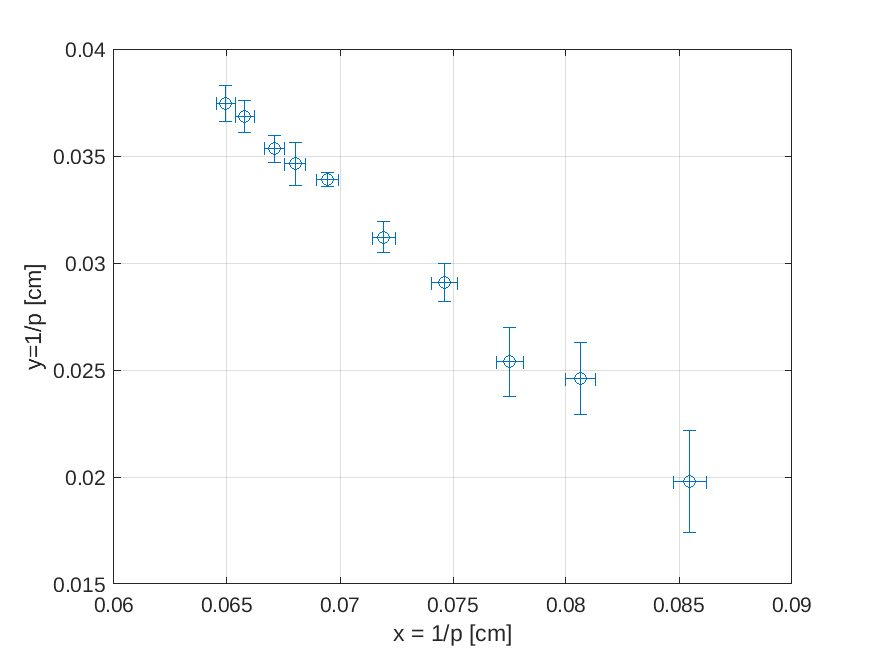
\includegraphics[width=0.7\textwidth]{scatter_linearized.png}
    \caption{Rappresentazione dei dati linearizzati}
    \label{fig:linearized}
\end{figure}

Dal momento che lo studio della linearità ha come obiettivo la stima della distanza della focale tramite best-fit, occorre indagare l'effettiva correlazione lineare per cui si calcola l'indice di Bravais-Pearson
\\
\begin{equation}
    r=\frac{\sum_{i=1}^n\left(x_i-\bar{x}\right)\left(y_i-\bar{y}\right)}{\sqrt{\sum_{i=1}^n\left(x_i-\bar{x}\right)^2 \sum_{i=1}^n\left(y_i-\bar{y}\right)^2}}
\end{equation}
\\
che applicato ai dati della Tabella \ref{tab:linearized} restituisce
\\
\begin{equation}
    r_0 = -0.997.
\end{equation}
\\
Al coefficiente $r_0$ si associa il seguente valore di probabilità \textit{p-value} o P (stimato tramite la funzione \texttt{corr()} di \texttt{MATLAB})
\\
\begin{equation}
    P(r_0) = 6.08 \cdot 10^{-10}
\end{equation}
\\
che, essendo $<< 0.01 = 1 \%$, lascia supporre una correlazione altamente significativa. Si procede dunque a determinare i coefficienti della retta di best-fit sfruttando il metodo dei minimi quadrati.
\\
\\
Come è possibile osservare dalla Figura \ref{fig:linearized} (o equivalentemente dalla Tabella \ref{tab:linearized}), le incertezze $\delta y$ sui punti $y$ non sono costanti, pertanto si è preferito effettuare un best-fit pesato e si sono determinati i parametri $A$ e $B$ introdotti in eq. \ref{eq:retta-generica}(rispettivamente, intercetta dell'asse delle ordinate e coefficiente angolare) come indicato dalle equazioni 8.37, 8.38, 8.93 (Taylor)

\begin{equation}
    A=\frac{\sum w x^2 \sum w y-\sum w x \sum w x y}{\Delta}
    \tag{8.37}
\end{equation}


\begin{equation}
    B=\frac{\sum w \sum w x y-\sum w x \sum w y}{\Delta}
    \tag{8.38}
\end{equation}
dove
\begin{equation}
    \Delta=\sum w \sum w x^2-\left(\sum w x\right)^2.
    \tag{8.39}
\end{equation}
\\
Le incertezze in $A$ e $B$ sono
\begin{equation}
    \begin{gathered}
        \qquad{\sigma_A=\sqrt{\frac{\sum w x^2}{\Delta}}}
        \qquad{\sigma_B=\sqrt{\frac{\sum w}{\Delta}}}.
    \end{gathered}
\end{equation}
\\
Applicando tali relazioni ai valori della Tabella \ref{tab:linearized}, si ottiene la retta di best-fit pesato (vd. Tabella \ref{tab:fit-params})
\\
\begin{equation}
    y = 0.094 - 0.87 x
    \label{eq:fit-pesato}
\end{equation}
\\
rappresentata dal segmento rosso della Figura \ref{fig:fit}. Si noti che i coefficienti dell'equazione \ref{eq:fit-pesato} sono stati indicati privi di incertezza per evitare di appesantire la notazione; si rimanda alla Tabella \ref{tab:fit-params} per la consultazione degli intervalli di incertezza dei parametri $A$ e $B$.
\\
Ritengo sia importante osservare che, essendo l'equazione linearizzata
\\
\begin{equation}
    \frac{1}{q} = \frac{1}{f} - \frac{1}{p} \; ,
\end{equation}
\\
il parametro $B$ dovrebbe risultare compatibile con il valore $-1$; tuttavia ciò non accade in quanto -1 non è compreso nell'intervallo $[B - \sigma_B, B + \sigma_B]$, infatti (vd. Tabella \ref{tab:fit-params})
\\
\begin{equation}
    B = -0.87 \pm 0.07 \Longrightarrow -1 \notin [-0.94,-0.80]
\end{equation}
\\
Rinviando al seguito lo studio di eventuali errori sistematici, si procede dunque alla determinazione del solo parametro $A$ eseguendo un adattamento dei minimi quadrati pesato e vincolato  (nel seguito indicato come \textit{best-fit pesato e vincolato}) avendo posto $B_0 = -1$
\\
\begin{equation}
 \qquad{A=\frac{\left(\sum_{i=1}^n w_i y_i\right)-\left(\sum_{i=1}^n w_i x_i\right) B_0}{\left(\sum_{i=1}^n w_i\right)}}
 \qquad{\sigma_A = \frac{\frac{\left(\sum_{i=1}^n w_i\left(y_i - B_0 x_i - A\right)^2\right)}{n-1}}{\left(\sum_{i=1}^n w_i\right)}}.
\end{equation}
\\
La retta di best-fit pesato e vincolato è rappresentata dalla linea gialla della Figura \ref{fig:fit} e ha equazione (vd. Tabella \ref{tab:fit-params})
\begin{equation}
    y = 0.1031 -x
    \label{eq:fit-vincolato}
\end{equation}

\begin{figure}[H]
    \centering
    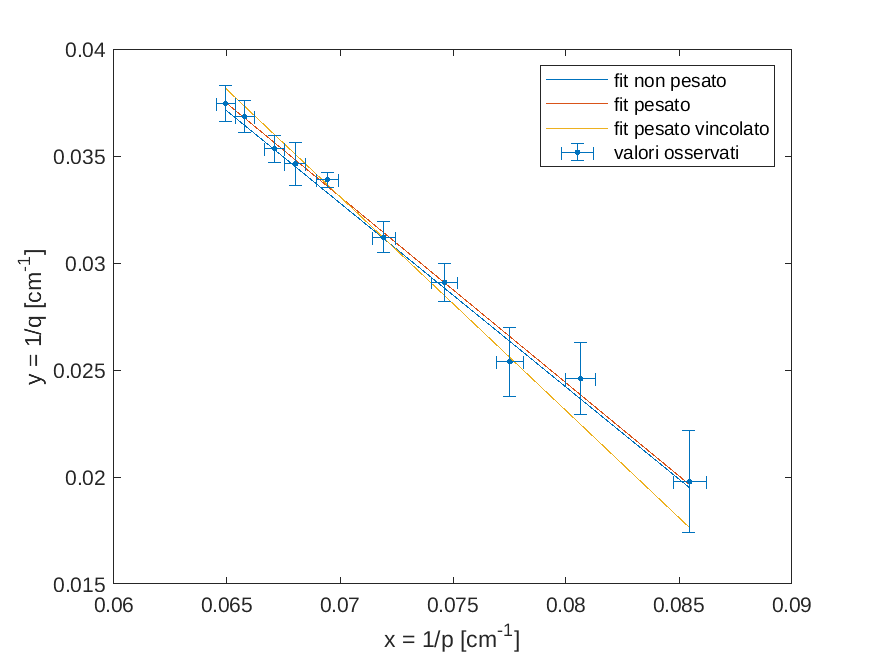
\includegraphics[width=0.8\textwidth]{fit.png}
    \caption{Metodo dei minimi quadrati}
    \label{fig:fit}
\end{figure}

\begin{longtable}{@{}llll@{}}
\toprule
Fit & $A \pm \sigma_A \; [cm^{-1}]$ & $B \pm \sigma_B$ & $\chi_{red}^2$ \tabularnewline
\midrule
non pesato, non vincolato & $0.093 \pm 0.002$ & $-0.86 \pm 0.03$ & 0.55 \tabularnewline
pesato, non vincolato & $0.094 \pm 0.005$ & $-0.87 \pm 0.07$ & 0.24 \tabularnewline
pesato e vincolato & $0.1031 \pm 0.0002$ & $-1$ & 0.74 \tabularnewline
\bottomrule
\label{tab:fit-params}
\\
\caption{Parametri dei fit $y = A +Bx$}
\end{longtable}

Per studiare l'adattamento e l'applicabilità ai dati (Tabella \ref{tab:linearized}) delle curve sopra descritte, si è calcolato il $\chi^2$ ridotto, nel seguito indicato con il simbolo $\chi_{red}^2$
\\
\begin{equation}
    \chi_{red}^2 = \frac{1}{n-s} \sum_{i=0}^n \left( \frac{y_i^{fit}-y_i}{\sigma_i} \right)^2
    \label{eq:chi}
\end{equation}
\\
dove: $n$ rappresenta il numero di punti, $s$ il numero di parametri della curva di fitting, $y_i^{fit}$ i valori assunti dalle funzioni lineari i cui parametri sono riportati in Tabella \ref{tab:fit-params}, $y_i$ le ordinate della Tabella \ref{tab:linearized}. Il denominatore del termine all'interno della sommatoria, a rigore, rappresenterebbe i soli contributi casuali delle incertezze $\delta y$; tuttavia, dal momento che non si hanno stime di tali valori, si farà uso delle $\delta y$ stesse (vd. Tabella \ref{tab:linearized}). I risultati dell'applicazione dell'equazione \ref{eq:chi} ai dati linearizzati sono consultabili nella Tabella \ref{tab:fit-params}; per completezza, tale parametro è stato determinato anche per il fit non pesato e non vincolato i cui parametri sono stati determinati sfruttando le equazioni 8.10, 8.11, 8.12, 8.15, 8.16, 8.17 (Taylor). Si osserva $\chi_{red}^2 < 1$ per ogni fit. In particolare i fit non vincolati restituiscono un $\chi_{red}^2$ minore di quello determinato considerando il fit vincolato (eq. \ref{eq:fit-vincolato}); si assume pertanto che quest'ultimo sia $\cong 1$ e si reputano i parametri di tale curva utili nella stima della distanza focale $f$ tramite best-fit.
\\ \\
Dalle equazioni \ref{eq:pqf-linearized} e \ref{eq:xy} si conclude infatti che l'intercetta $A$ (assunta uguale a $0.1031 \pm 0.0002 \; cm^{-1}$) coincide con il reciproco della distanza focale $f$, pertanto
\begin{equation}
    A = \frac{1}{f} \Longrightarrow f = \frac{1}{A}
    \label{eq:f-da-A}
\end{equation}
a cui cui attribuiamo incertezza
\begin{equation}
    \delta f = \sqrt{\left ( \frac{\partial f}{\partial A}\sigma_A \right ) ^2} = \left | \frac{\partial f}{\partial A}\sigma_A \right | = \frac{\sigma_A}{A^2}.
\end{equation}
Concludiamo dunque che la stima della distanza focale $f$ da best-fit (pesato e vincolato) sia
\begin{equation}
    f_{fit} = 9.70 \pm 0.02 \; cm
    \label{eq:f-fit-value}
\end{equation}
\subsubsection{Ingrandimento}
Calcolo l'ingrandimento $m_1$ attraverso le misure della lunghezza della fenditura dell'immagine
\begin{equation}
    i = \frac{l_{sup} + l_{inf}}{2}
\end{equation}

L'incertezza su $i$ si assume come il semintervallo in cui l'immagine appare nitida
\begin{equation}
    \delta i = \frac{|l_{sup}-l_{inf}|}{2}
\end{equation}
\begin{equation}
    m_1 = \frac{i}{o}
\end{equation}
\\
con $o = cost = 1.850 \pm 0.005 cm$ misurata col calibro
\\
\begin{equation}
    \delta m_1 = \sqrt{\left(\frac{\partial m}{\partial i}\delta i\right )^2 + \left( \frac{\partial m}{\partial o} \delta o \right )^2}\\
    = \sqrt{\left( \frac{1}{o} \delta i \right)^2+ \left(\frac{i}{o^2}\delta o \right)^2}
\end{equation}
\\
Le prime tre colonne di questa tabella sono le stesse riportate nelle tabelle precedenti ma accostate a i per facilitarne la lettura 
\\
\begin{longtable}[]{@{}lllll@{}}
    \toprule
    Measure ID & $l_{inf}$ & $l_{sup}$ & $i$ & $m_1 \pm \delta m_1$ \tabularnewline
    & $\pm 0.005 \; [cm]$ & $\pm 0.005 \; [cm]$ & [cm] \tabularnewline
    \midrule
    \endhead
    C1M1  & 6.360 & 7.850 & $7.1 \pm 0.7$   & $3.8 \pm 0.4$ \tabularnewline
    C1M2  & 5.090 & 6.230 & $5.7 \pm 0.6$   & $3.1 \pm 0.3$ \tabularnewline
    C1M3  & 5.065 & 6.095 & $5.6 \pm 0.5$   & $3.0 \pm 0.3$ \tabularnewline
    C1M4  & 4.235 & 4.850 & $4.5 \pm 0.3$   & $2.5 \pm 0.2$ \tabularnewline
    C1M5  & 3.985 & 4.320 & $4.2 \pm 0.2$   & $2.24 \pm 0.09$ \tabularnewline
    C1M6  & 3.600 & 3.275 & $3.4 \pm 0.2$   & $1.86 \pm 0.09$ \tabularnewline
    C1M7  & 3.265 & 3.890 & $3.6 \pm 0.3$   & $1.9 \pm 0.2$ \tabularnewline
    C1M8  & 3.410 & 3.535 & $3.47 \pm 0.06$ & $1.88 \pm 0.03$ \tabularnewline
    C1M9  & 3.150 & 3.995 & $3.6 \pm 0.4$   & $1.9 \pm 0.2$ \tabularnewline
    C1M10 & 3.000 & 3.285 & $3.1 \pm 0.1$   & $1.7 \pm 0.08$ \tabularnewline
    \bottomrule
    \label{tab:ingrandimento}
    \\
    \caption{Dati ingrandimento da i e o}
 \end{longtable}

Si è poi calcolato l'ingrandimento $m_2$ come rapporto tra $q$ e $p$.
\begin{equation}
    m_2 = \frac{q}{p}
\end{equation}

\begin{equation}
    \delta m_2 = \sqrt{\left(\frac{\partial m}{\partial q}\delta q\right )^2 + \left( \frac{\partial m}{\partial p} \delta p \right )^2}\\
    = \sqrt{\left( \frac{1}{p} \delta q \right)^2+ \left(\frac{q}{p^2}\delta p \right)^2}.
\end{equation}
\\
Di seguito si affiancano i valori di $m$ ottenuti tramite i due metodi sopra descritti

\begin{longtable}[]{@{}llll@{}}
    \toprule
    Measure ID & $m_1 \pm \delta m_1$ & $m_2 \pm \delta m_2$ & $\Delta m$ \tabularnewline
    \midrule
    \endhead
    C1M1 & $3.8   \pm 0.4 $ & $4.3  \pm 0.5 $ & 0.5 \tabularnewline
    C1M2 & $3.1   \pm 0.3 $ & $3.3  \pm 0.2 $ & 0.2 \tabularnewline
    C1M3 & $3.0   \pm 0.3 $ & $3.1  \pm 0.2 $ & 0.1 \tabularnewline
    C1M4 & $2.5   \pm 0.2 $ & $2.57 \pm 0.08$ & 0.1 \tabularnewline
    C1M5 & $2.24  \pm 0.09$ & $2.31 \pm 0.06$ & 0.1 \tabularnewline
    C1M6 & $1.86  \pm 0.09$ & $2.05 \pm 0.03$ & 0.2 \tabularnewline
    C1M7 & $1.9   \pm 0.2 $ & $1.96 \pm 0.06$ & 0.1 \tabularnewline
    C1M8 & $1.88  \pm 0.03$ & $1.90 \pm 0.04$ & 0.02 \tabularnewline
    C1M9 & $1.9   \pm 0.2 $ & $1.79 \pm 0.04$ & 0.1 \tabularnewline
    C1M10& $1.70  \pm 0.08$ & $1.73 \pm 0.04$ & 0.0 \tabularnewline
    \bottomrule
    \label{tab:ms}
    \\
    \caption{Ingrandimento, confronto}
 \end{longtable}


Di seguito si confrontano visualmente i valori ottenuti tramite i due metodi da cui si osserva come gli intervalli delle misure e delle loro incertezze si sovrappongano per 9 misure su 10. Pertanto le misure indirette risultano tutte compatibili ad eccezione della sesta misura.

I dati in Tabella \ref{tab:ms} sono stati rappresentati in \ref{fig:ms} comprensivi di intervallo di incertezza per facilitare la valutazione della sovrapposizione

\begin{figure}[H]
    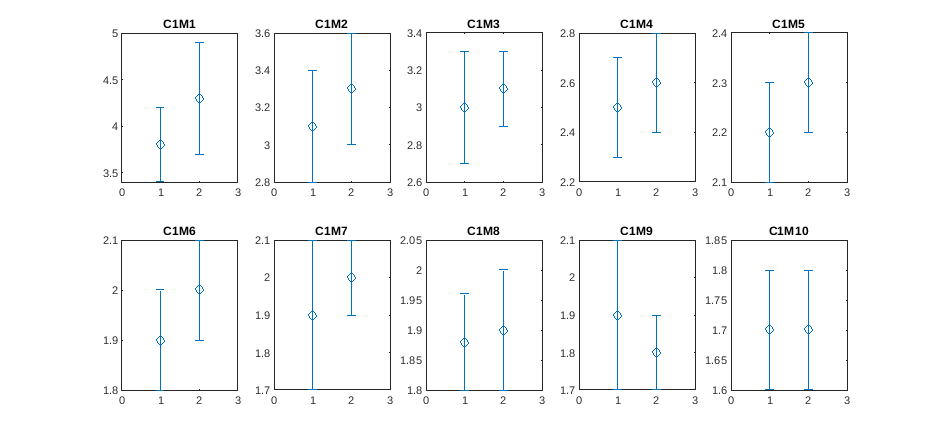
\includegraphics[width=1\textwidth]{ms.png}
    \caption{Valori dell'ingrandimento $m$. Sull'asse delle $x$ l'indice corrispondente al metodo di calcolo}
    \label{fig:ms}
\end{figure}

\subsubsection{Metodo di Bessel}
L'ultima stima di $f$ riportata in questo studio sarà effettuata sfruttando il metodo di Bessel. Avendo introdotto $x_o$ e $x_s$ in Tabella \ref{tab:dati-bessel}, nella configurazione in cui $p = q$ e $m = 1$, la distanza oggetto-schermo sarà
\begin{equation}
    D = |x_o - x_s|
\end{equation}
a cui si attribuisce l'incertezza
\begin{equation}
    \delta D = 2\delta s
\end{equation}
con $\delta s = 0.1 \; cm$ che corrisponde all'incertezza sulle misure delle posizioni per questa configurazione.
\\ \\
Si determina quindi la distanza focale e relativa incertezza dalle relazioni
\begin{equation}
    \qquad{f_b = \frac{D}{q}}
    \qquad{\delta f_b} = \frac{\delta D}{4}
\end{equation}
che applicate ai dati della Tabella \ref{tab:dati-bessel}, con $D = 39.6 \pm 0.2 \; cm$, restituiscono i seguenti valori
\begin{equation}
    f_b = 9.90 \pm 0.05 \; cm.
\end{equation}

\subsection{Potenza della lente}
Avendo stimato la distanza focale $f$, è possibile determinare la potenza $\Pi$ della lente dalla definizione
\begin{equation}
    \Pi = \frac{1}{f}.
\end{equation}
Se $f$ è espressa in metri, infatti, il suo reciproco rappresenta $\Pi$ espressa in diottrie. 
\\ \\
L'incertezza sulla potenza $\Pi$ sarà
\begin{equation}
    \delta \Pi = \left | \frac{\partial \Pi}{\partial f} \delta f \right | = \frac{\delta f}{f^2}.
\end{equation}
eventualmente moltiplicata per un fattore 100 nel caso in cui $f$ sia espressa in cm (come sopra).
\\ \\
Procediamo alla stima di tale grandezza considerando i valori di $\bar{f_d}$, $f_{fit}$ e $f_b$ avendo eseguito le opportune equivalenze. 
\\ \\
Essendo $\bar{f_d}$ la media pesata delle distanze focali (espresse in cm) ottenute in modo diretto (vd. equazioni \ref{eq:media-pesata-f} e \ref{eq:f-diretta-media-pesata}), determino
\begin{equation}
    \Pi_1 = \frac{1}{\frac{\bar{f_d}}{100}} = \frac{100}{\bar{f_d}}.
    \label{eq:potenza-1}
\end{equation}
Considerando il reciproco della $f_{fit}$ (anch'essa espressa in cm) ottenuta tramite best-fit lineare pesato e vincolato (vd. equazioni \ref{eq:f-da-A}, \ref{eq:f-fit-value})
\begin{equation}
    \Pi_2 = \frac{1}{\frac{f_{fit}}{100}} = \frac{100}{f_{fit}} = \frac{100}{\frac{1}{A}} = 100 A.
    \label{eq:potenza-2}
\end{equation}
Infine, si è stimata la potenza anche della distanza focale $f_b$ ottenuta tramite il metodo di Bessel
\begin{equation}
    \Pi_3 = \frac{1}{\frac{f_{b}}{100}} = \frac{100}{f_{b}}.
    \label{eq:potenza-3}
\end{equation}
I risultati sono stati riportati in Tabella \ref{tab:potenza}
\begin{longtable}{@{}llll@{}}
\toprule
Metodo & Equazione & $\Pi \pm \delta \Pi$ & $\frac{\delta \Pi}{\Pi}$ \tabularnewline
\midrule
1 & \ref{eq:potenza-1} & $10.31 \pm 0.03$ & 0.29\% \tabularnewline
2 & \ref{eq:potenza-2} & $10.31 \pm 0.02$ & 0.19\% \tabularnewline
3 & \ref{eq:potenza-3} & $10.10 \pm 0.05$ & 0.5\% \tabularnewline
\bottomrule
\label{tab:potenza}
\\
\caption{Potenza della lente}
\end{longtable}
Si è proceduto al calcolo della media pesata
\begin{equation}
    \qquad{\Pi_w = \frac{\sum_{i=1}^{3} w_i \Pi_i}{\sum_{i=1}^{3} w_i }} \; ,
    \qquad{\delta \Pi_w = \sqrt{\frac{1}{\sum_{i=1}^{3} w_i}}}\; ,
    \qquad{w_i = \frac{1}{(\delta \Pi_i)^2}}
    \label{eq:media-pesata-potenza}
\end{equation}
\\
da cui si conclude che la migliore stima della potenza $\Pi$ della lente è
\\
\begin{equation}
    \Pi_w = 10.29 \pm 0.02 \; m^{-1}
    \label{eq:potenza-media-pesata-value}
\end{equation}

\begin{figure}[H]
    \centering
    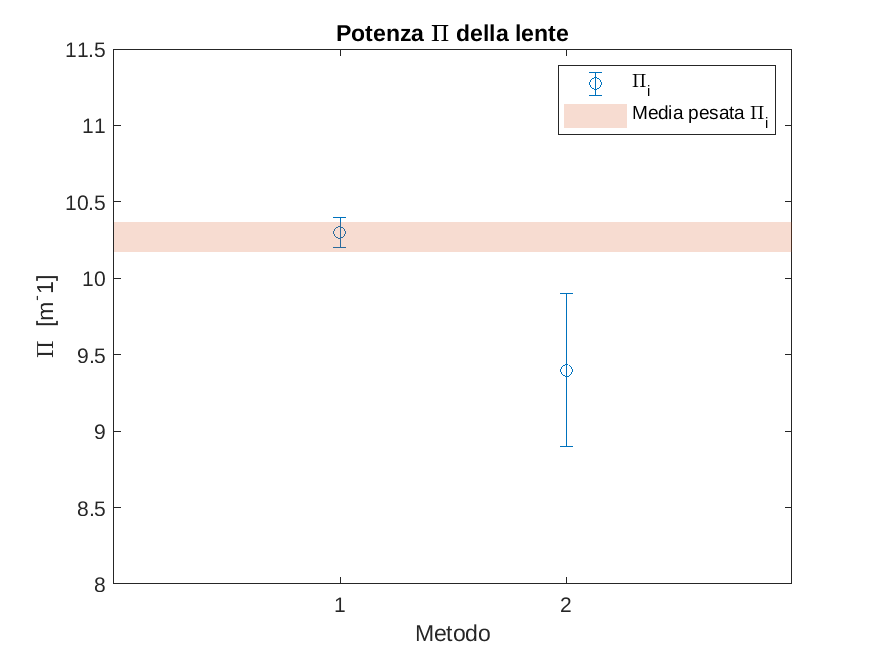
\includegraphics[width=0.7\textwidth]{potenza-lente.png}
    \caption{Stima della potenza $\Pi$ della lente tramite diversi metodi}
    \label{fig:potenza}
\end{figure}


\subsection{Valutazione di eventuali errori sistematici}
Detta $\delta s = 0.05 \; cm$ l'incertezza sulle posizioni per questa configurazione (vd. Tabella \ref{tab:dconf3}) per ogni distanza $D$ oggetto-schermo sono stato determinati: 

\begin{itemize}
    \item il punto medio $x_m$ di D
    \begin{equation}
    \qquad{x_m = \frac{x_o + x_s}{2}}
    \qquad{\Delta x_m = \frac{\delta s}{\sqrt{2}}} \;
    \end{equation}
    
    \item la distanza $s$ tra il punto medio $x_m$ e il punto $x_{l1}$, coincidente con l'estremo inferiore dell'intervallo delle posizioni della lente per cui l'immagine fosse nitida
    \begin{equation}
        \qquad{s = |x_m - x_{l1}|}
        \qquad{\Delta s = \sqrt{(\Delta x_m)^2 + (\delta s)^2}}
    \end{equation}

    \item la distanza $d$ tra il punto medio $x_m$ e il punto $x_{l2}$, coincidente con l'estremo superiore dell'intervallo delle posizioni della lente per cui l'immagine fosse nitida
    \begin{equation}
        \qquad{d = |x_m - x_{l2}|}
        \qquad{\Delta d = \sqrt{(\Delta x_m)^2 + (\delta s)^2} = \Delta s}.
    \end{equation}
\end{itemize}
Si è poi valutata la differenza
\begin{equation}
    \qquad{\eta = |s-d|}
    \qquad{\Delta \eta = \sqrt{(\Delta s)^2 + (\Delta d)^2}} = \Delta s \sqrt{2}.
\end{equation}
I simboli $\Delta$ delle relazioni precedenti rappresentano le incertezze sulle misure per evitare di modificare la notazione per cui $\delta s$ indica l'incertezza sulle posizioni.
\\
In Tabella \ref{tab:sd} è possibile consultare i valori di $x_m$, $s$, $d$ e $\eta$

\begin{longtable}{@{}lllll@{}}
\toprule
Measure ID & $x_m$ & s & d & $\eta$ \tabularnewline
& $\pm 0.04 \; [cm]$ & $\pm 0.08 \; [cm]$ & $\pm 0.08 \; [cm]$ & $\pm 0.1 \; [cm]$ \tabularnewline
\midrule
C3M1 & 32.05 & 7.90 & 6.85 & 1.0 \tabularnewline
C3M2 & 32.30 & 7.95 & 6.75 & 1.2 \tabularnewline
C3M3 & 32.55 & 7.90 & 7.10 & 0.8 \tabularnewline
C3M4 & 32.80 & 8.55 & 7.40 & 1.1 \tabularnewline
C3M5 & 33.05 & 9.15 & 7.80 & 1.3 \tabularnewline
C3M6 & 33.30 & 9.25 & 7.35 & 1.9 \tabularnewline
C3M7 & 33.40 & 9.30 & 8.30 & 1.0 \tabularnewline
C3M8 & 33.55 & 9.40 & 8.55 & 0.8 \tabularnewline
C3M9 & 33.70 & 9.70 & 8.55 & 1.1 \tabularnewline
C3M10 & 33.80 & 9.70 & 9.05 & 0.6 \tabularnewline
C3M11 & 33.95 & 10.00 & 9.10 & 0.9 \tabularnewline
\bottomrule
    \label{tab:sd}
    \\
    \caption{Stima errori sistematici}
 \end{longtable}
Nessuno degli $\eta$ dellta Tabella \ref{tab:sd} risulta compatibile con lo zero: si rilevano quindi errori sistematici. Avendo assunto che la distribuzione delle $\eta$ sia gaussiana per $n$ tendente a $\infty$ (Figura \ref{fig:eta}), si sono stimati il valor medio $\bar{\eta}$ e la deviazione standard $\sigma_{\eta}$
\begin{figure}[H]
    \centering
    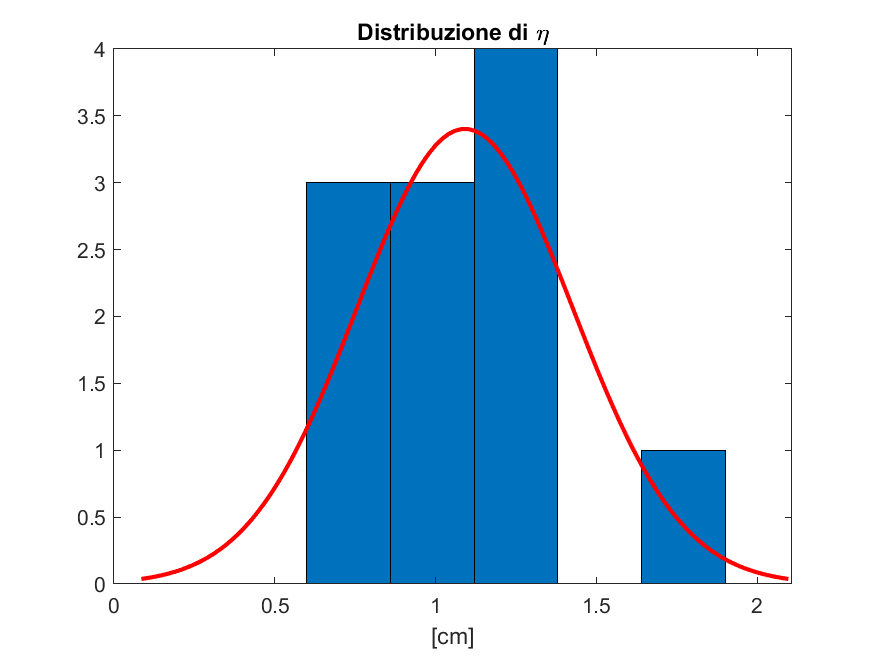
\includegraphics[width=0.7\textwidth]{eta.png}
    \caption{Istogramma degli $\eta$}
    \label{fig:eta}
\end{figure}


\begin{equation}
    \bar{\eta} = \frac{1}{n} \sum_i^n \eta_i = 1.1 \; cm
    \label{eq:eta-sist}
\end{equation}

\begin{equation}
    \sigma_{\eta} = \sqrt{\frac{{\sum_{i=1}^{11}(\eta_i - \overline{\eta})^2}}{{10}}} = 0.3 \; cm.
\end{equation}
\\
La miglior stima del contributo sistematico alle incertezze sulle misure della distanza focale $f$ è costituita da $\bar{\eta} \pm \sigma_{\eta}$; pertanto, detta $\Delta f$ l'incertezza sulla distanza focale $f$ e considerando le incertezze $\delta f$ precedentemente propagate, si ha 
\begin{equation}
    \Delta f = \delta f + \bar{\eta}.
\end{equation}

\section{Conclusione}
Come esposto nei paragrafi precedenti, si è pervenuti alla stima della distanza focale $f$ tramite 3 metodi. Non considerando i contributi sistematici all'incertezza di $f$, i valori della distanza focale risultano essere molto precisi (con un errore relativo $\delta f/f \leq 0.5\%$).

 \begin{longtable}{@{}llll@{}}
\toprule
Metodo & Simbolo & Descrizione & $f \pm \delta f$ \tabularnewline
\midrule
1 & $\bar{f_d}$ & media pesata & $9.70 \pm 0.03$ \tabularnewline
2 & $f_{fit}$ & best-fit pesato e vincolato & $9.70 \pm 0.02$ \tabularnewline
3 & $f_b$ & bessel & $9.90 \pm 0.05$ \tabularnewline
    \bottomrule
    \label{tab:fs-no-sist}
    \\
    \caption{Valori di $f$ ottenuti tramite diversi metodi di misura e analisi}
 \end{longtable}

In tali condizioni, si assume che la migliore stima di $f$ sia la media pesata $f_w$ a cui si attribuisce incertezza $\delta f_w$ (intervallo rappresentato dalla banda rossa della Figura \ref{fig:fs})
\\
\begin{equation}
    \qquad{f_w = \frac{\sum_i w_i f_i}{\sum_i w_i}}
    \qquad{w_i = \frac{1}{\delta f_i ^2}}
    \qquad{\delta f_w = \sqrt{\frac{1}{\sum_i w_i}}}.
\end{equation}
\\
Si conclude dunque
\begin{equation}
    f_w = 9.72 \pm 0.02 \; cm
\end{equation}
\\
\begin{figure}[H]
    \centering
    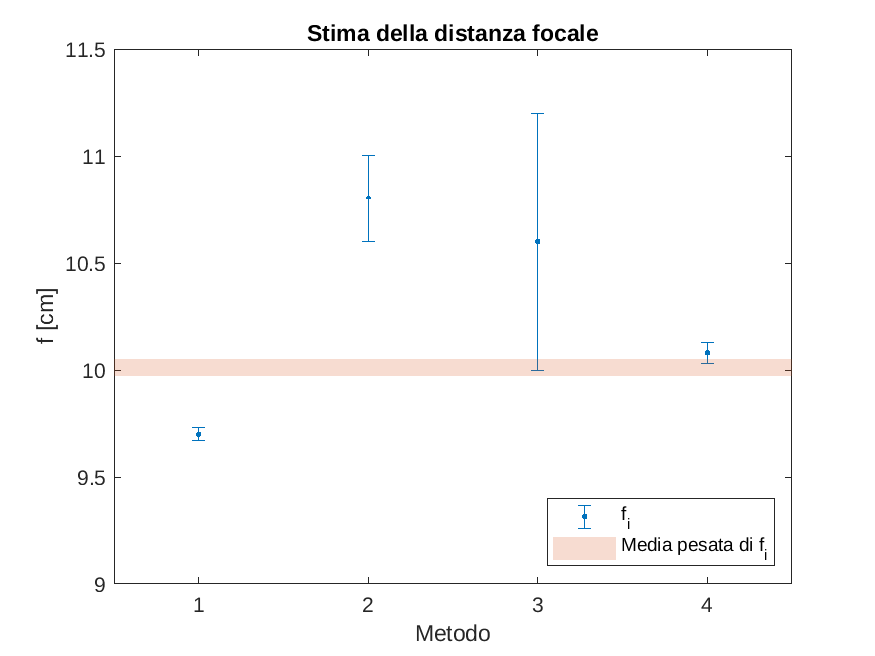
\includegraphics[width=0.7\textwidth]{fs.png}
    \caption{Distanza focale (incertezza priva di contributi sistematici)}
    \label{fig:fs}
\end{figure}
Tuttavia è importante osservare come, mentre gli intervalli di $\bar{f_d}$ e $f_{fit}$ risultano compatibili sia tra di loro che con l'intervallo della media pesata $[f_w-\delta f_q, f_w + \delta f_w]$, lo stesso non avviene per $f_b$.
\\ \\
Se si includono i contributi sistematici che sono stati rilevati nei paragrafi precedenti (vd. equazione \ref{eq:eta-sist}), si perde l'elevata precisione e si perviene alla stessa stima di $f$ per tutti i metodi utilizzati (vd. equazione \ref{f-end}) che risultano inevitabilmente compatibili.
\begin{figure}[H]
    \centering
    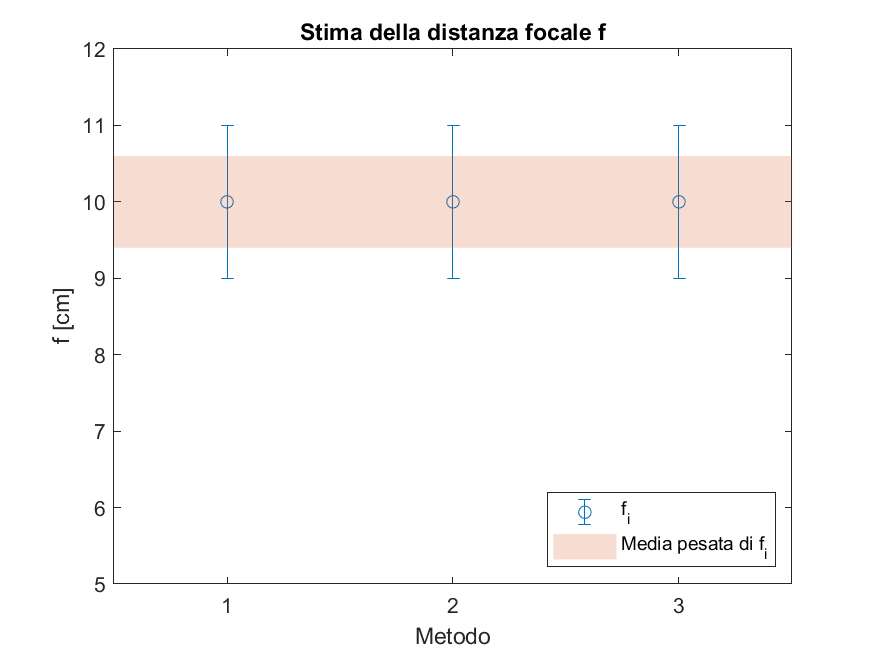
\includegraphics[width=0.7\textwidth]{fs-sist.png}
    \caption{Distanza focale}
    \label{fig:fs-sist}
\end{figure}
In ultima analisi è possibile concludere come la migliore stima di $f$ sia rappresentata da
\begin{equation}
    f_w \pm \Delta f = 10 \pm 1 \; cm
    \label{f-end}
\end{equation}
che, avendo un errore relativo del 10\%, può essere comunque ritenuta soddisfacente.

\section{Note aggiuntive}

\subsection{Data availability}
I dati grezzi che sono stati raccolti per la realizzazione di questo studio sono disponibili in formato open. Questi, nel rispetto della definizione degli standard internazionali, sono stati pubblicati:
\begin{itemize}
    \item in formato neutro e \textit{machine-readable} (\texttt{CSV});
    \item con \href{https://creativecommons.org/licenses/by/4.0/}{Licenza CC-BY 4.0} che ne consente il riutilizzo.
\end{itemize}
La piattaforma scelta per la distribuzione di tali contenuti è GitHub: i dati sono stati depositati nel  repository \texttt{dennisangemi/lab2-exam} raggiungibile al seguente indirizzo\\\href{https://github.com/dennisangemi/lab2-exam}{https://github.com/dennisangemi/lab2-exam/tree/main/data}.
\\ \\
The data that support the findings of this study are openly available in dennisangemi/lab2-exam GitHub Repository at \href{https://github.com/dennisangemi/lab2-exam}{https://github.com/dennisangemi/lab2-exam/tree/main/data} under \href{https://creativecommons.org/licenses/by/4.0/}{CC-BY 4.0 license}.

\subsection{Code availability}
Analogamente a quanto scritto per la distribuzione dei dati grezzi, anche il codice MATLAB che è stato utilizzato per analizzare i dati è disponibile nel repository GitHub dennisangemi/lab2-exam GitHub Repository al link
\href{https://github.com/dennisangemi/lab2-exam/tree/main/scripts}{https://github.com/dennisangemi/lab2-exam/tree/main/scripts}.
\\ \\
The MATLAB code written to get the findings of this study is openly available in dennisangemi/lab2-exam GitHub Repository at \href{https://github.com/dennisangemi/lab2-exam/tree/main/scripts}{https://github.com/dennisangemi/lab2-exam/tree/main/scripts}

\subsection{Software utilizzati}
\begin{itemize}
    \item \textbf{Google Sheets}: Data Collection
    \item \textbf{MATLAB}: Data Analysis
    \item \textbf{GitHub}: Resource sharing
    \item \textbf{Figma}: Images designing
\end{itemize}

\section{Bibliografia e sitografia}
\begin{itemize}
    \item Taylor,~ J. (1999).~\emph{Introduzione all'analisi degli errori: Lo
  studio delle incertezze nelle misure fisiche.~}Zanichelli
    \item Bevington, P. (2002).~\emph{Data Reduction and Error Analysis for the Physical Sciences.~} McGraw-Hill Education ~
    \item Malthe-Sørenssen, A. (2015). \emph{Elementary Mechanics Using Matlab: A Modern Course Combining Analytical and Numerical Techniques}. Springer
    \item Mazzoldi, P., Nigro, M., Voci, C. (2001). \emph{Fisica. Meccanica, termodinamica (Vol. 1)}. Edises
    \item Mencuccini, C., Silvestrini, V. (1998). \emph{Fisica 2. Elettromagnetismo-ottica. Corso di fisica per le facoltà scientifiche. Con esempi ed esercizi }. Liguori Editore
    \item Costa, S. (2012). \emph{Misura della distanza focale di una lente convergente} \href{https://cms333.ct.infn.it/~costa}{https://cms333.ct.infn.it/~costa}
    \item Costa, S. (2023). \emph{Lezione n. 22. Misure, strumenti di misura, incertezze sperimentali} \href{https://cms333.ct.infn.it/~costa}{https://cms333.ct.infn.it/~costa}
\end{itemize}

\end{document}
